\documentclass[twocolumn]{article}
\usepackage{graphicx}

\title{Conditional 3D Environment Generation Using Deep Adversarial Networks}

\author{Tim Whitaker \\ Colorado State University}

\begin{document}

	\maketitle
	
	\section{Abstract}
	
	We introduce a method and application for generating 3D environments with generative adversarial networks. The outputs from our networks are able to be imported into popular three dimensional modeling software like Unreal, Unity and Blender. We've created a simple and easy to use web based interface to allow a user to control the output of the generated environment by painting with predefined brushes that represent terrain varieties: mountains, hills, terraces, plains, and rivers.
	
	\section{Introduction}

	This project explores the usage of conditional generative adversarial networks to synthesize 3 dimensional environments.
	
	The motivations for this project are to make it easier for game, world or environment designers to create realistic environments procedurally while giving the designer more control over the results.
	
	We aim to create a simple and easy to use GUI interface for a user to paint a 2 dimensional semantically significant image map. We then pass the user created image map through a generative adversarial network trained on elevation data gathered from the Earth in order to generate a realistic terrain heightmap that approximately represents the user defined map. The resulting heightmap produced from the neural network can then be uploaded into any of the popular 3 dimensional rendering softwares including Unity, Unreal, Blender or World Machine.
	
	\section{Background}
	
	This project explores the new paradigm of 3 dimensional procedurally generated content via machine learning.
		
	\subsection{Procedural Content Generation}
	
	Procedural content generation is an algorithmic and stochastic process used in art, games, music and film. As a paradigm for content generation, it is used to increase replayability, variability, flexibility and reduce production cost, effort storage space \cite{summerville2017procedural}.

	\subsection{Generative Adversarial Networks}
	
	Neural networks have become a pervasive part of computer science. It allows for a powerful model of learning patterns from complex datasets. Generative adversarial networks work by synthesizing novel data according to patterns it learns in the training set. We evaluate two models of conditional generative adversarial networks to achieve image to image translation.
	
	We are going to evaluate two implementations of a specialized form of generative adversarial networks designed to perform conditional image to image translation. The two models we are using are called Pix2Pix and CycleGAN.
	
	Both Pix2Pix and CycleGAN are based on the deep convolutional generative adversarial network architecture proposd by Radford et al. in 2015 \cite{radford2015unsupervised}.
	
	\subsubsection{Pix2Pix}	
	
	Pix2Pix introduces a a generalized approach to image to image translation problems.  Their model learns not only a mapping between input and output images, but it also learns a loss function between the two image datasets. This allows this model to be used for a variety of image tasks that would originally need very different model and loss configurations \cite{isola2016imagetoimage}.
	
	\subsubsection{CycleGAN}
	
	CycleGAN introduces the idea of cycle consistency loss. It works by measuring the loss of a mapping from one distribution to another and then back to the original distribution again. This approach allows for good generalization and the advantage of not needing specifically paired images in the training distributions. This can save a lot of time in building large datasets, but it can lose out on the specificity offered by Pix2Pix \cite{zhu2017unpaired}.

	\subsection{Related Work}

	Nvidia GauGAN.
	
	\section{Methodology}
	
	In this section we go over all of the pieces of work that went in to this project.
	
	\subsection{User Interface Application}
	
	The user interface is a web based javascript application that allows a user to paint a semantically significant image using predefined brushes. We include tools to change th brush size and export or clear the image. The canvas size is 512 x 512 pixels, and these images are resized automatically when passed to our neural network.

	\begin{figure}[h!]
	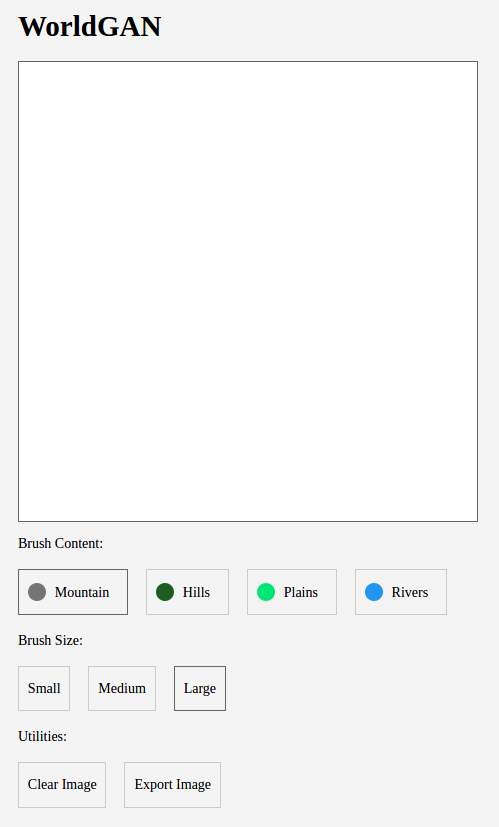
\includegraphics[width=1\columnwidth]{ui.png} 
	\caption{The user interace application}
	\end{figure}
	
	The backend is powered by a Flask API. We set up an endpoint to be able to evaluate a drawn image on our trained models.
	
	\subsection{The Dataset}
	
	Generative adversarial networks need a good amoount of training data to output good results and a key objective of this project is to generate realistic results. This leads to an interesting challenge of putting together a realistic yet sizable dataset. In order to achieve this, we use terrain data of the earth as opposed to fictional or manufactured terrain data. In the next two sections we go into the methodology behind building the dataset.

	\subsubsection{Training Data}
	
	I used an interactive open source map tool that visualizes elevation data gathered from Mapzen's global elevation service \cite{richardson2016mapzen}.
	
	I then built a program that controls a headless browser using an open source library developed by Google called puppeteer. This script loads a random coordinate, checks if the coordinate is over land and if so, then we save an image of the elevation data at that coordinate. We resize the saved image to be 512 x 512 pixels.
	
	We then started manually building the usermap training set using the WorldGAN user interface application. For each image in the heightmap training set, We paint a usermap to represent that heightmap, using the semantically significant brushes that most closely match the terrain (mountains, hills, plains, rivers, and terraces). This process is a subjective one and all usermaps were painted by myself. This does bias the model to produce images according to how I read the heightmaps.

	After this process we are left with 259 paired usermaps and heightmaps. We group all of these together into a batch to be trained on.

	Creating the usermaps by hand is quite time consuming, and I wanted to experiment with models trained on a large dataset. We accomplish this by augmenting our first batch with simple transformations in order to artificially increase the number of images we can train on. Image augmentations are a well researched and effective appoach to improving neural network performance \cite{perez2017effectiveness}.
	
	We performed 5 operations on each usermap and heightmap. We mirror horizontally, flip vertically, rotate 90 derees, rotate 180 degrees, and rotate 270 degrees.	All of the resulting images are gathered into a second batch and we end up with 1548 paired images (a 5x increase).
	
	Before training the networks, we need to perform one more preprocessing step. Pix2Pix requires paired images to be combined into a single side by side image. We stack each pair of usermap and heightmap and save these images into separate batches spcifically for Pix2Pix. Each resulting image is 1024 x 512 pixels. CycleGAN does not need this preprocessing step and can be trained on images in different directories.
			
	\subsubsection{Test Data}
	
	The test data is a collection of 10 usermaps I drew that are designed to be representative of a variety of environments a user might draw. These 5 environments include mountainous regions, hilly regions, flat regions and combined regions.
	
	\subsection{Training The Models}
	
	We trained a total of 4 models. Pix2Pix and CycleGAN on both the original batch of training data and the augmented batch. The training was performed on my desktop GPU enabled PC. The relevant specifications include an Nvidia GTX 1080ti GPU with 11 GB of memory, an Intel i7 8700k processor, a 500GB solid state hard drive, and 32 GB of RAM.
	
	Both models are built on top of the PyTorch framework \cite{paszke2019pytorch}.
	
	\subsubsection{Pix2Pix}
	~1 hour training time.
	~4 hours training time.
	
	\subsubsection{CycleGAN}
	~4 hours training time.
	~24 hours training time.

	\subsection{Visualizations Using 3D Software}
	
	Visualizations of results with 3d software.

	\section{Results}
	
	\subsection{Visualizations Using 3D Software}

	\section{Conclusion}
	
	\subsection{Future Work}

	\bibliographystyle{plain}
	\bibliography{references}	
  
\end{document}